

\section{Gérer les stocks de composants pour réaliser des drones}
L'entreprise \texttt{SuperDrone} réalise le montage et la vente de drones.\\

\begin{minipage}{.7\textwidth}%
Les composants utiles pour réaliser un drone sont :
\begin{itemize}
\item le châssis ;
\item les 4 moteurs ;
\item les 4 hélices ;
\item la batterie ;
\item le contrôleur de vol ;
\item ESC 4 en 1 pour les 4 moteurs (Electronic Speed Controler) ;
\item la plaque de distribution de puissance (PDB Power Distribution Board).
\end{itemize}
\end{minipage}%
\hfill
\begin{minipage}{.3\textwidth}%
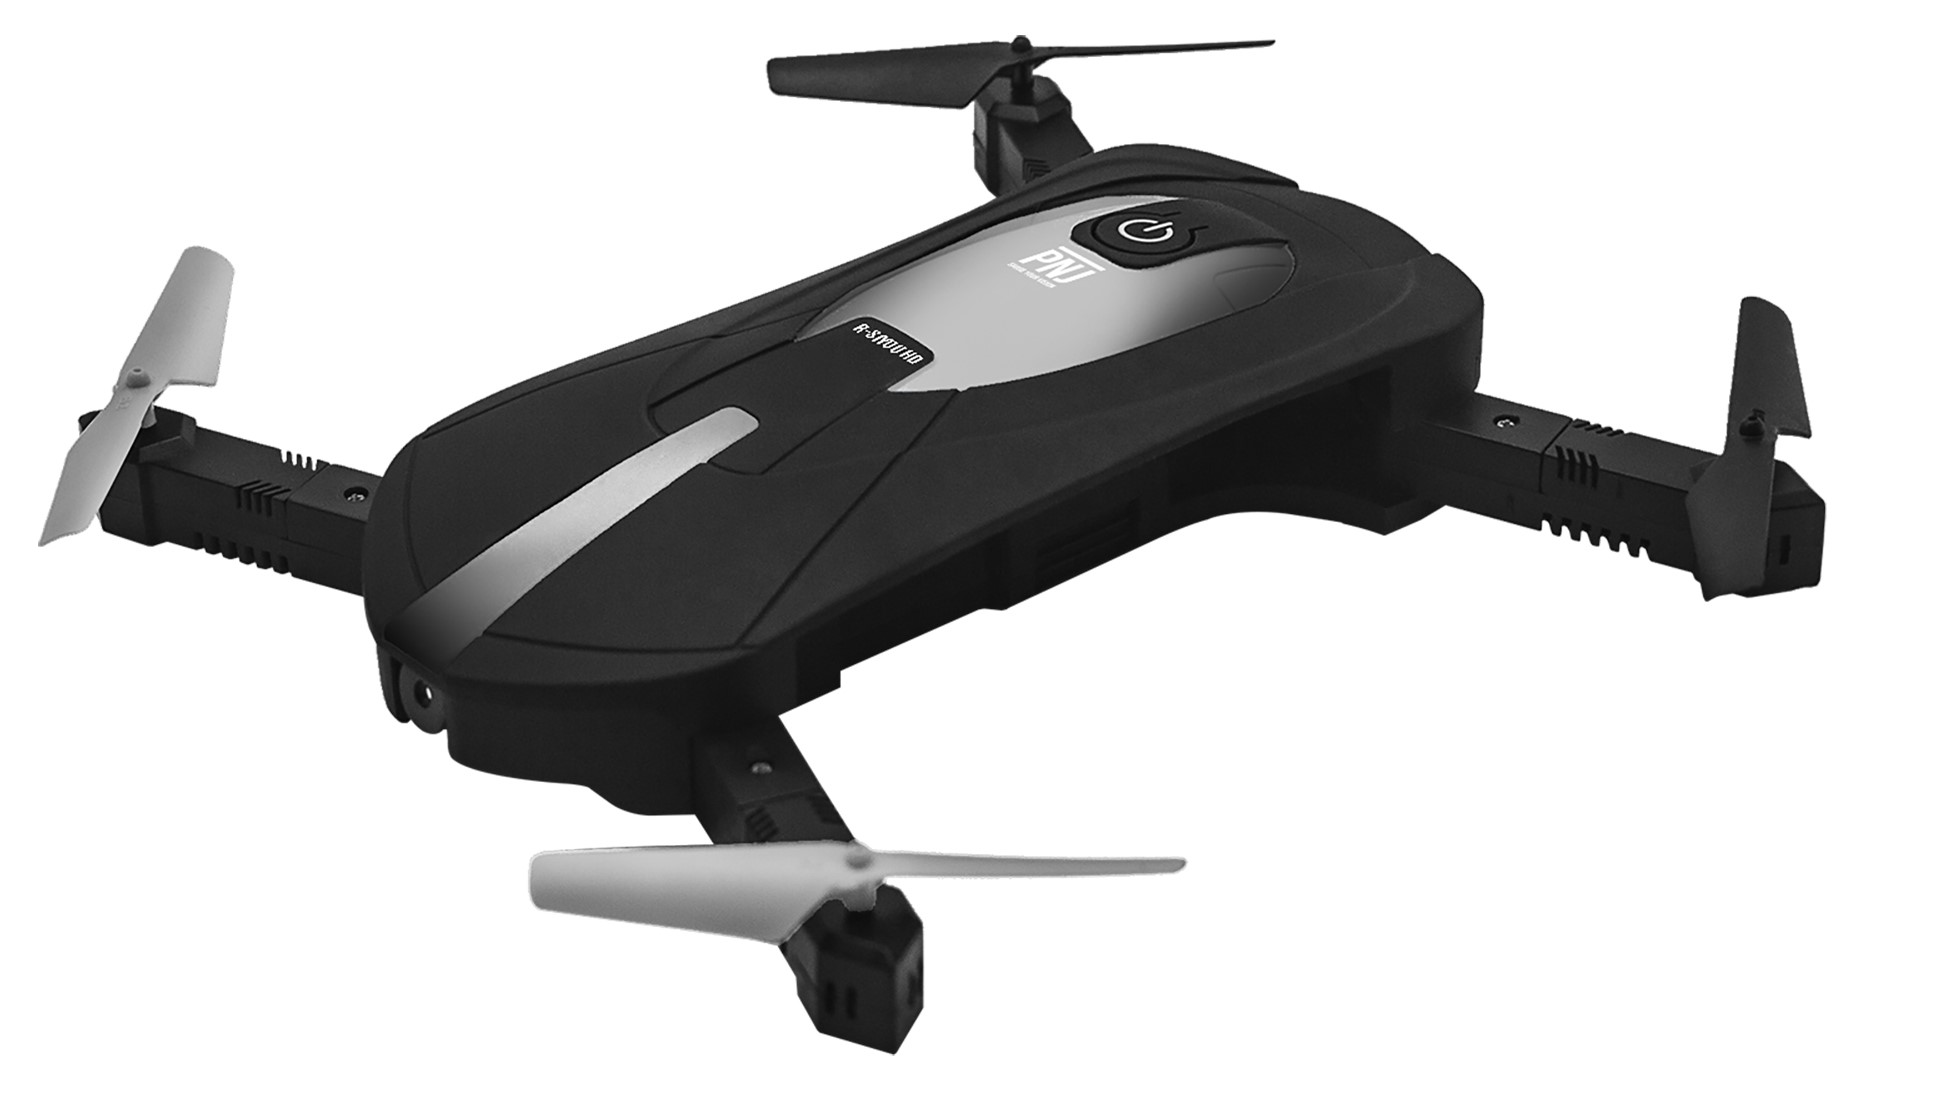
\includegraphics[width=\textwidth]{drone.jpg}
\end{minipage}
Des composants en option sont aussi disponibles (caméra, radiocommande, chargeur, buzzer, leds...) et ne seront pas traités ici.\\

Dans le fichier \texttt{drone.py} donné, vous trouverez 4 dictionnaires dont les clés sont les noms des composants et les valeurs représentent le nombre de composants nécessaire :

\begin{lstlisting}
drone={'moteur':4,'chassis':1,'controleurVol':1,'ESC4en1':1,'batterie':1,'helice':4,
'plaqueDeDistribution':1}
stock={'chassis':0,'moteur':25,'helice':36,'controleurVol':12,'ESC4en1':8,'batterie':20,
'plaqueDeDistribution':7}
limiteMin={'chassis':2,'moteur':8,'helice':8,'controleurVol':2,'ESC4en1':2,'batterie':2,
'plaqueDeDistribution':2}
limiteMax={'chassis':15,'moteur':60,'helice':60,'controleurVol':15,'ESC4en1':15,'batterie':30,
'plaqueDeDistribution':15}
\end{lstlisting}

\begin{itemize}
\item \texttt{drone}, correspond aux composants nécessaires à la réalisation d'un drone. Les clés étant les composants et les valeurs le nombre de composant pour un drone;
\item \texttt{stock}, correspond au stock à l'instant considéré;
\item \texttt{limitMin}, correspond aux valeurs limites basses du stock pour déclencher une commande;
\item \texttt{limitMax}, correspond aux valeurs limites hautes pour reconstituer le stock et pour définir le nombre de composants à commander.
\end{itemize}

\begin{obj}
\'Ecriture d'un programme qui permette de générer les commandes de composants utiles pour assurer la réalisation des drones attendus par les clients sans avoir de rupture de stock.\\
On utilisera des objets de type \texttt{dict}.
\end{obj}

\subsection*{Réaliser un drone}


\question{
\'Ecrire la fonction \texttt{realiser1Drone(drone:dict, stock:dict)} qui prend pour argument les dictionnaires \texttt{drone} et \texttt{stock} et qui renvoie un booléen, \texttt{True} si le stock est suffisant pour réaliser un drone, \texttt{False} sinon.
}

\subsection*{Gérer le stock de composants}

\question{
\'Ecrire la fonction \texttt{destocker(D:dict, S:dict)} qui prend pour argument les dictionnaires \texttt{D} des composants du drone et \texttt{S} du stock et qui retire du stock le nombre de composants utiles pour réaliser un drone. Cette fonction ne renvoie rien. Le dictionnaire \texttt{S} est modifié par effet de bord.
}



Lorsque le stock devient insuffisant, une commande est passée et le stock est ré-évalué.

\question{
\'Ecrire la fonction \texttt{stocker(C:dict, S:dict)} qui prend pour argument les dictionnaires \texttt{C} correspondant à la commande et \texttt{S} du stock et qui ajoute au stock le nombre de composants commandés. Cette fonction ne renvoie rien. Le dictionnaire \texttt{S} est modifié par effet de bord, le dictionnaire \texttt{C} n'est pas modifié.
}

\subsection*{Passer une commande}
Une commande est passée quand le stock d'un composant est à la limite basse (valeur incluse). Les composants qui n'ont pas atteint la limite basse ne sont pas commandés.

\question{
\'Ecrire la fonction \texttt{commanderComposant(S:dict,limiteMin:dict,limiteMax:dict)} qui prend pour argument les dictionnaires \texttt{S} du stock, \texttt{limiteMin} et \texttt{limiteMax} et qui renvoie un dictionnaire \texttt{commande} permettant de reconstituer le stock.
}

\subsection*{Gestion automatique}
Dans la semaine, l'entreprise \texttt{SuperDrone} reçoit les commandes de drones de 4 clients sous la forme d'une liste, \texttt{listeCommande}=\verb![!3,1,5,2\verb!]!.

\question{
\'Ecrire la fonction \texttt{satisfaireClient(listeCommande:list,drone:dict,stock:dict,\\
limiteMin:dict,limiteMax:dict)} qui prend pour argument une liste de commande de drones, les dictionnaires \texttt{drone}, \texttt{stock}, \texttt{limiteMin} et \texttt{limiteMax} et qui affiche l'état du stock après chaque réalisation d'un drone ainsi que les commandes successives.
}
